\documentclass[12pt]{article}
\usepackage[margin=1in]{geometry}
\usepackage{float}
\usepackage{listings}
\usepackage{graphicx}
\usepackage{placeins}
\usepackage[nottoc]{tocbibind} %Adds "References" to the table of contents
\usepackage{graphicx}
\setlength\parindent{0pt}

\lstset{
	frame=tb,
	showstringspaces=false,
	columns=flexible,
	breaklines=true,
	breakatwhitespace=true
}

\begin{document}
\pagenumbering{gobble}
\begin{titlepage}
   \vspace*{\stretch{1.0}}
   \begin{center}
      \textsc{\Huge プログラミング実験第三}\\ [1cm]
      \textsc{\Huge TinyJavaScript コンパイラの作り直し}\\ [2cm]
      \large\textit{\huge 1311216}\\
      \large\textit{\huge Rathore Amogh\\}
      \large\textit{\huge 岩崎研究室\\}
   \end{center}
   \vspace*{\stretch{2.0}}
\end{titlepage}


\tableofcontents

\newpage
\pagenumbering{arabic}

\section{はじめに}
\subsection{背景}
TinyJavaScript は JavaScript の一部機能を制限んしたサブセットのことである\cite{jscompiler}。TinyJavaScriptの元のコンパイラは Mozilla の SpiderMonkey Parser API \cite{spidermonkey}を使用していた。しかし、SpiderMonkey Parser は絶えてしまって、TinyJavaScript のコンパイラの開発も続けられなくなった。だから、TinyJavaScript コンパイラを新しいパーサを使用して作りなおす必要が出てきた。このレポートは TinyJavaScript コンパイラを Node JS で作る実験について述べる。

\subsection{実験の目的}
この実験ではTinyJavaScriptのコンパイラをNodeJSとEsprima (ECMAScript Parsing Infrastructure for Multipurpose Analysis) \cite{esprima}を使用して実装する。それで、コンパイラの作り方と構造について学習する。最後に、実験で作った新しいコンパイラとTinyJavaScriptの\cite{jscompiler}で述べてるコンパイラの比較を行う。

\subsection{実装の方針}
実装にはEsprimaというECMAScript\cite{ecmascript} Parserを使用する。JavaScriptはECMAScriptのdialectであるので、ECMAScriptのパーサはJavaScriptの構文に対して正しくパーシングをされる。参考のため\cite{jscompiler}で述べてるTinyJavaScript Compilerの実装を使う。もう少し具体的に言うと、Esprimaを使ってTinyJavaScriptのソースコードを抽象構文木に変換する。それから、抽象構文木をトラバースしてSSJSVM(これについて後で述べる)の命令列を生成する。

\section{TinyJavaScript と SSJSVM}
\subsection{TinyJavaScript}
TinyJavaScriptはJavaScriptの以下の機能をサポートしない \cite{jscompiler}
\begin{itemize}
\item with 文
\item delete 文
\item グローバル変数宣言時の var の省略
\item for in 文
\item switch 文
\item 名前付きの関数定義
\end{itemize}

\subsection{SSJSVM}
SSJSVM は Server-side JavaScript Virtual Machine の略称である。すなわち、サーバで動くJavaScriptの仮想機械のことである。本実験では、TinyJavaScriptのソースコードをSSJSVMの命令列に変換するコンパイラを作る。

\section{パーサの選び方}
実験の目的はTinyJavaScriptのコンパイラを新しいパーサ(SpiderMonkey 1.6でないパーサ)を使用して作るということである。だから、プログラミングを始める前にパーサを選ぶ必要がある。以下の特徴を持つパーサを使いたい。

\begin{enumerate}
\item ECMAScript の新しいバージョンをサポートする
\item 構文解析を正しくやってくれる
\item 使いやすい
\item ドキュメントとサポートがいい
\end{enumerate}

いろいろ調べた結果、2つの案が出てきた。

\begin{itemize}
\item ECMAScriptの文法を揃えてANTLR\cite{antlr} (ANother Tool for Language Recognition)を使ってパーサを生成する
\item Esprima を使う
\end{itemize}

ANTLRを使用するとANTLR用の文法が必要となる。その文法はいろいろなソースがインターネットで提供してるが、オフィシャルではないので正しさは保証できない。あとドキュメントなども全然提供されてなくて、使いにくいと判断した。ところで、Esprimaはとてもアクチブなプロジェクトであって、投稿者が多い。だから、最後にEsprimaを使うと決める。

\section{Esprima}
Esprima \cite{esprima}はJavaScriptで書かれてるECMAScriptのパーシングインフラストラクチャである。Esprimaの主な特徴は以下のとおりである\cite{esprima}。

\begin{itemize}
\item ECMAScript 6 (ECMA-262 \cite{ecmascript}) 全体をサポート
\item Estree プロジェクトの標準を対応する構文木フォーマット
\item よくテストされたパーサ \cite{esprimaTests}
\item オープンソース \cite{esprimaGitHub}
\end{itemize}

\section{コンパイラの設計}
本実験で作るコンパイラは、ソースコードを3つの段階で仮想機械の命令列に変換する。その段階は以下の通りである。

\begin{figure}
\centering
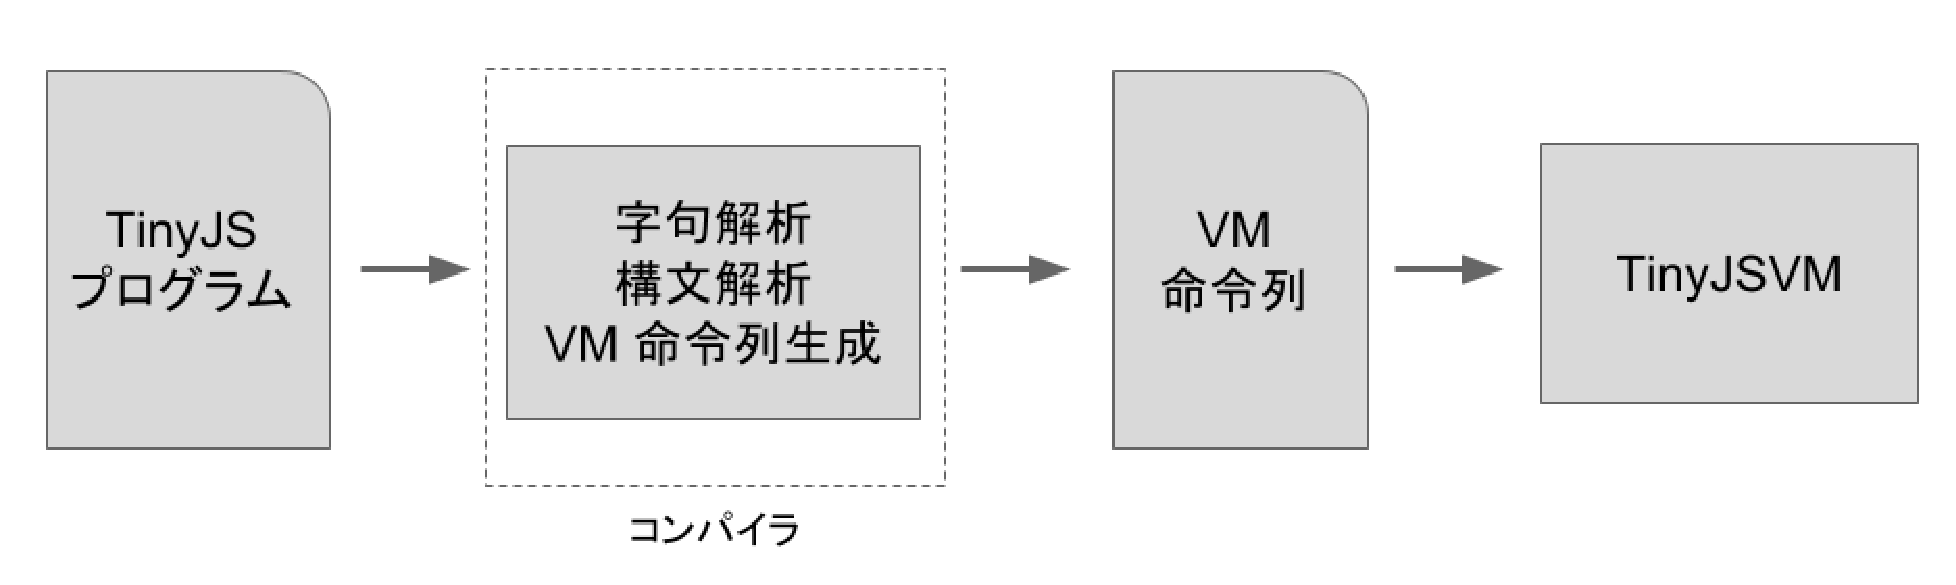
\includegraphics[scale=0.5]{process.eps}
\caption{コンパイルの3つの段階}
\end{figure}
\FloatBarrier

\begin{enumerate}
\item ソースコードの字句解析を行う
\item 字句列から抽象構文木を生成する
\item 抽象構文木を仮想機械の命令列に変換する
\end{enumerate}

本実験で使うEsprimaパーサは段階1と段階2の処理を行ってくれる。Esprimaは抽象構文木をJSオブジェクトにして返す。

\section{コンパイラの実装}

\section{評価}

\section{終わりに}

\newpage
\begin{thebibliography}{9}
\bibitem{jscompiler}
高田 祥. \textit{ARM 上で動作する JavaScript 処理系の実装}. 電気通信大学 電気通信学部
情報工学科 ソフトウェア学講座. January, 2011.
\bibitem{spidermonkey}
SpiderMonkey 1.6 \newline
http://www-archive.mozilla.org/js/spidermonkey/release-notes/
\bibitem{esprima}
Esprima \newline
http://esprima.org/
\bibitem{esprimaTests}
Esprimaのテスト情報 \\
http://esprima.org/test/ci.html
\bibitem{esprimaGitHub}
Esprimaのソースコード \\
https://github.com/jquery/esprima
\bibitem{ecmascript}
ECMAScript \newline
http://www.ecma-international.org/publications/standards/Ecma-262.htm
\bibitem{antlr}
ANTLR \newline
http://www.antlr.org/
\bibitem{estree}
EStree プロジェクト \\
https://github.com/estree/estree
\end{thebibliography}

\end{document}
